
\documentclass[11pt,a4paper]{article}
%\documentclass[PICOReport.tex]{extragalacticsci.tex}
\def\simlt{\mathrel{\rlap{\lower 3pt\hbox{$\sim$}}\raise 2.0pt\hbox{$<$}}}
\def\simgt{\mathrel{\rlap{\lower 3pt\hbox{$\sim$}} \raise2.0pt\hbox{$>$}}}

\usepackage{amssymb,amsmath,times}

\usepackage{color}

\usepackage{graphicx}

\usepackage{fancyhdr}

\usepackage{multirow}

\usepackage{cite}

\usepackage{color}

\usepackage{natbib}

\usepackage{acronym}

%\usepackage{aas_macros}

\def\araa{Ann.~Rev.~Astr.~Ap.}

% define formatting

%\pagestyle{empty}

\parindent=0pt

\topmargin=0.in \headheight=0in \headsep=-0.1in \textheight=9.2in

\textwidth=6.5in \oddsidemargin=0in


\setlength{\floatsep}{0.5\floatsep}

\setlength{\textfloatsep}{0.5\textfloatsep}

\setlength{\intextsep}{0.5\intextsep}

\setlength{\floatsep}{0.5\floatsep}

\setlength{\dblfloatsep}{0.5\dblfloatsep}

\setlength{\dbltextfloatsep}{0.5\dbltextfloatsep}




% define spacings
\def\p{\smallskip}
\def\sp{\vspace{0.15in}}
\def\spa{\vspace{0.3in}}
\def\spaa{\vspace{0.5in}}
\def\spaaa{\vspace{0.7in}}

% define shorthands for latex commands
\def\bei{\begin{itemize}}
\def\eei{\end{itemize}}

% define commonly used symbols
\def\et{{\it et al.\ }}
\def\degr{$^{\circ}$}
\def\arcsec{$^{\prime\prime}$}
\def\pp{\pi}

% define various names
\def\usk{ }
\def\max{MAX}
\def\maxima{MAXIMA}
\def\boom{BOOMERanG}
\def\arch{Archeops}
\def\maxboom{\maxima/\boom}
\def\planck{{\it Planck}}
\def\combat{COMBAT}
\def\cmb{CMB}
\def\cmba{CMBA}
\def\tic{Ticra}
\def\codef{CODE5}
\def\forecast{FORECAST}
\def\maxipol{MAXIPOL}
\def\hwp{HWP}
\def\ahwp{AHWP}
\def\wmap{WMAP}
\def\igb{IGB}
\def\apex{APEX}
\def\ebex{EBEX}
\def\squid{SQUID}
\def\ld{LD}
\def\ldii{LD-II}
\def\blast{BLAST}
\def\pb{\sc polarbear}
\def\pbsa{{\sc polarbear}/SA}
\def\spttg{SPT3G}
\def\ebextw{EBEX2013}
\def\ebexsk{EBEX-IDS}
\def\litebird{LiteBIRD}
\def\bicep{BKA}
\def\biceptwo{BICEP2}
\def\dfmux{DFMux}
\def\xsixf{$\times$64}
\def\xones{$\times$16}
\newcommand{\core}{\textit{\negthinspace CORE\/}}

% for systematics section
\newcommand{\suffix}{pdf} % for pdflatex
\newcommand{\pico}{PICO}
\newcommand{\prang}{\ensuremath{\alpha}}% Polarisation Rotation Angle
\newcommand{\arcmin}{\ensuremath{'}}
\newcommand{\degree}{\ensuremath{^o}}
\newcommand{\fsky}{f_{\rm sky}}
\newcommand{\EFH}[1]{\textcolor{red}{$\dagger${[#1]}$\dagger$}}


%define physics and cosmological notations
\def\het{$^{3}$He}
\def\hef{$^{4}$He}
\def\lnt{lN$_{2}$}
\def\wn{cm$^{-1}$}
\def\omeg{$\Omega$}
\def\omegb{$\Omega_{b}$}
\def\hubble{$H_{0}$}
\def\lamb{$\Lambda$}
\def\cl{$C_{\ell}$}
\def\micron{$\mu$m}
\def\microk{$\mu{\mbox{K}}$}
\def\microkrtsec{$\mu{\mbox{K}}\sqrt{\mbox{sec}}$}
\def\microkprthz{$\mu{\mbox{K}}/\sqrt{\mbox{Hz}}$}
\def\wattrthz{${\mbox{Watt}}\sqrt{\mbox{Hz}}$}
\def\voltprthz{${\mbox{Volt}}/\sqrt{\mbox{Hz}}$}
\def\sintheta{\mbox{$\sin\theta$}}
\def\bceti{$\beta$-ceti}
\def\etad{$\eta$-draconis}
\def\ruo2{RuO$_{2}$}
\def\tdot{$\dot{\theta}$}
\def\taub{$\tau_{b}$}
\def\degsq{deg$^2$}

% define polarization symbols parameters
\def\It{$I_{t}$}  
\def\sq{$Q$}
\def\su{$U$}
\def\dsu{$\Delta U$}
\def\dsq{$\Delta Q$}
\def\TT{$C_l^{\rm TT}$}
\def\TE{$C_l^{\rm TE}$}
\def\EE{$C_l^{\rm EE}$}
\def\BB{$C_l^{\rm BB}$}

% define math and vectors

\def\mathrelfun#1#2{\lower3.6pt\vbox{\baselineskip0pt\lineskip.9pt
  \ialign{$\mathsurround=0pt#1\hfil##\hfil$\crcr#2\crcr\sim\crcr}}}
\def\simlt{\mathrel{\mathpalette\mathrelfun <}}
\def\simgt{\mathrel{\mathpalette\mathrelfun >}}

\def\hatx{{\bf \hat n}}
\def\hatnprime{{\bf \hat n'}}
\def\hatnone{{\bf \hat n}_1}
\def\hatntwo{{\bf \hat n}_2}
\def\hatni{{\bf \hat n}_i}
\def\hatnj{{\bf \hat n}_j}
\def\vecx{{\bf x}}
\def\veck{{\bf k}}
\def\hatx{{\bf \hat x}}
\def\hatk{{\bf \hat k}}
\def\hatz{{\bf \hat z}}
\def\VEV#1{{\left\langle #1 \right\rangle}}
\def\cP{{\cal P}}
\def\noise{{\rm noise}}
\def\pix{{\rm pix}}
\def\map{{\rm map}}
\long\def\comment#1{}

% \newcommand{\beq}{\begin{equation}}
% \newcommand{\eeq}{\end{equation}}
% \newcommand{\bea}{\begin{eqnarray}}
% \newcommand{\eea}{\end{eqnarray}}
\newcommand\PRL{{\it Phys.~Rev.~Lett.}}
\newcommand\prl{{\it Phys.~Rev.~Lett.}}
\newcommand\ApJ{{\it Ap.~J.}}
\newcommand\apj{{\it Ap.~J.}}
\newcommand\ApJL{{\it Ap.~J.~Lett.}}
\newcommand\apjl{{\it Ap.~J.~Lett.}}
\newcommand\ApJS{{\it Ap.~J.~Suppl.}}
\newcommand\apjs{{\it Ap.~J.~Suppl.}}
\newcommand\PR{{\it Phys.~Rev.}}
\newcommand\PL{{\it Phys.~Lett.}}
\newcommand\MNRAS{{\it MNRAS}}
\newcommand\mnras{{\it MNRAS}}
\newcommand\MNRASL{{\it MNRAS\ Lett.}}
\newcommand\AnA{{\it Astron.~Astrophys.}}
\newcommand\BAAS{{\it Bull.~Am.~Astron.~Soc.}}
\newcommand\NP{{\it Nucl.~Phys.}}
\newcommand\RMP{{\it Rev.~Mod.~Phys.}}
\newcommand\ARAA{{\it ARAA}}
\newcommand\prd{{\it Phys.~Rev.~D.}}
\newcommand\plb{{\it Phys.~Lett.~B.}}
\newcommand\ao{{\it Appl.~Optics}}
\newcommand\aap{{\it Astron.~Astrophys.}}
\newcommand\aaps{{\it Astron.~Astrophys.~Suppl.}}
\newcommand\pasp{{\it Proc.~Ast.~Soc.~Pac.}}
\newcommand\josa{{\it J.~Opt.~Soc.~Am.}}
\newcommand\phr{{\it Phys. Reports}}
\newcommand\aj{{\it Astronomical Journal}}
\newcommand\jcap{{\it JCAP}}
\newcommand\apss{{\it ApSS}}

\newcommand{\comred}[1]{\textcolor{red}{#1}}
\newcommand{\comblue}[1]{\textcolor{blue}{#1}}

% Let's you define a command for both text and math mode. 
\newcommand{\wisk}[1]{{\ifmmode{#1}\else{$#1$}\fi}}



%subfiles






\begin{document}



\bibliographystyle{unsrt}






\def\mission{CMB Probe\ }

%% %simple case: 2 authors, same institution
%% \author{A. Uthor}
%% \author{and A. Nother Author}
%% \affiliation{Institution,\\Address, Country}

% %________________________________________________________________


\begin{figure*}
%\vskip-3cm
\begin{center}
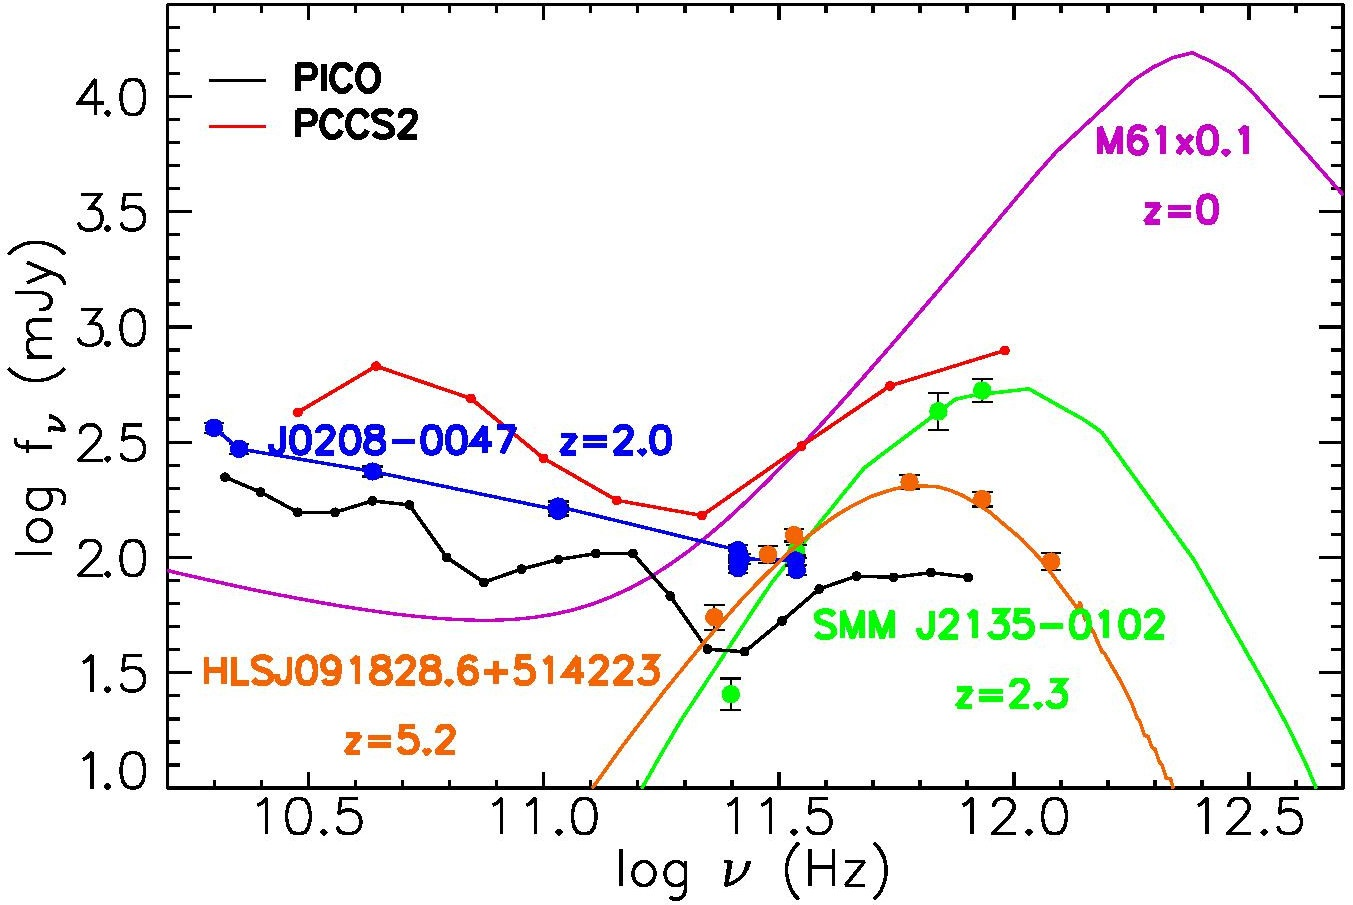
\includegraphics[width=0.48\columnwidth, trim={0 0 0 0cm}, clip]{fig_SED3_PICO.jpg}
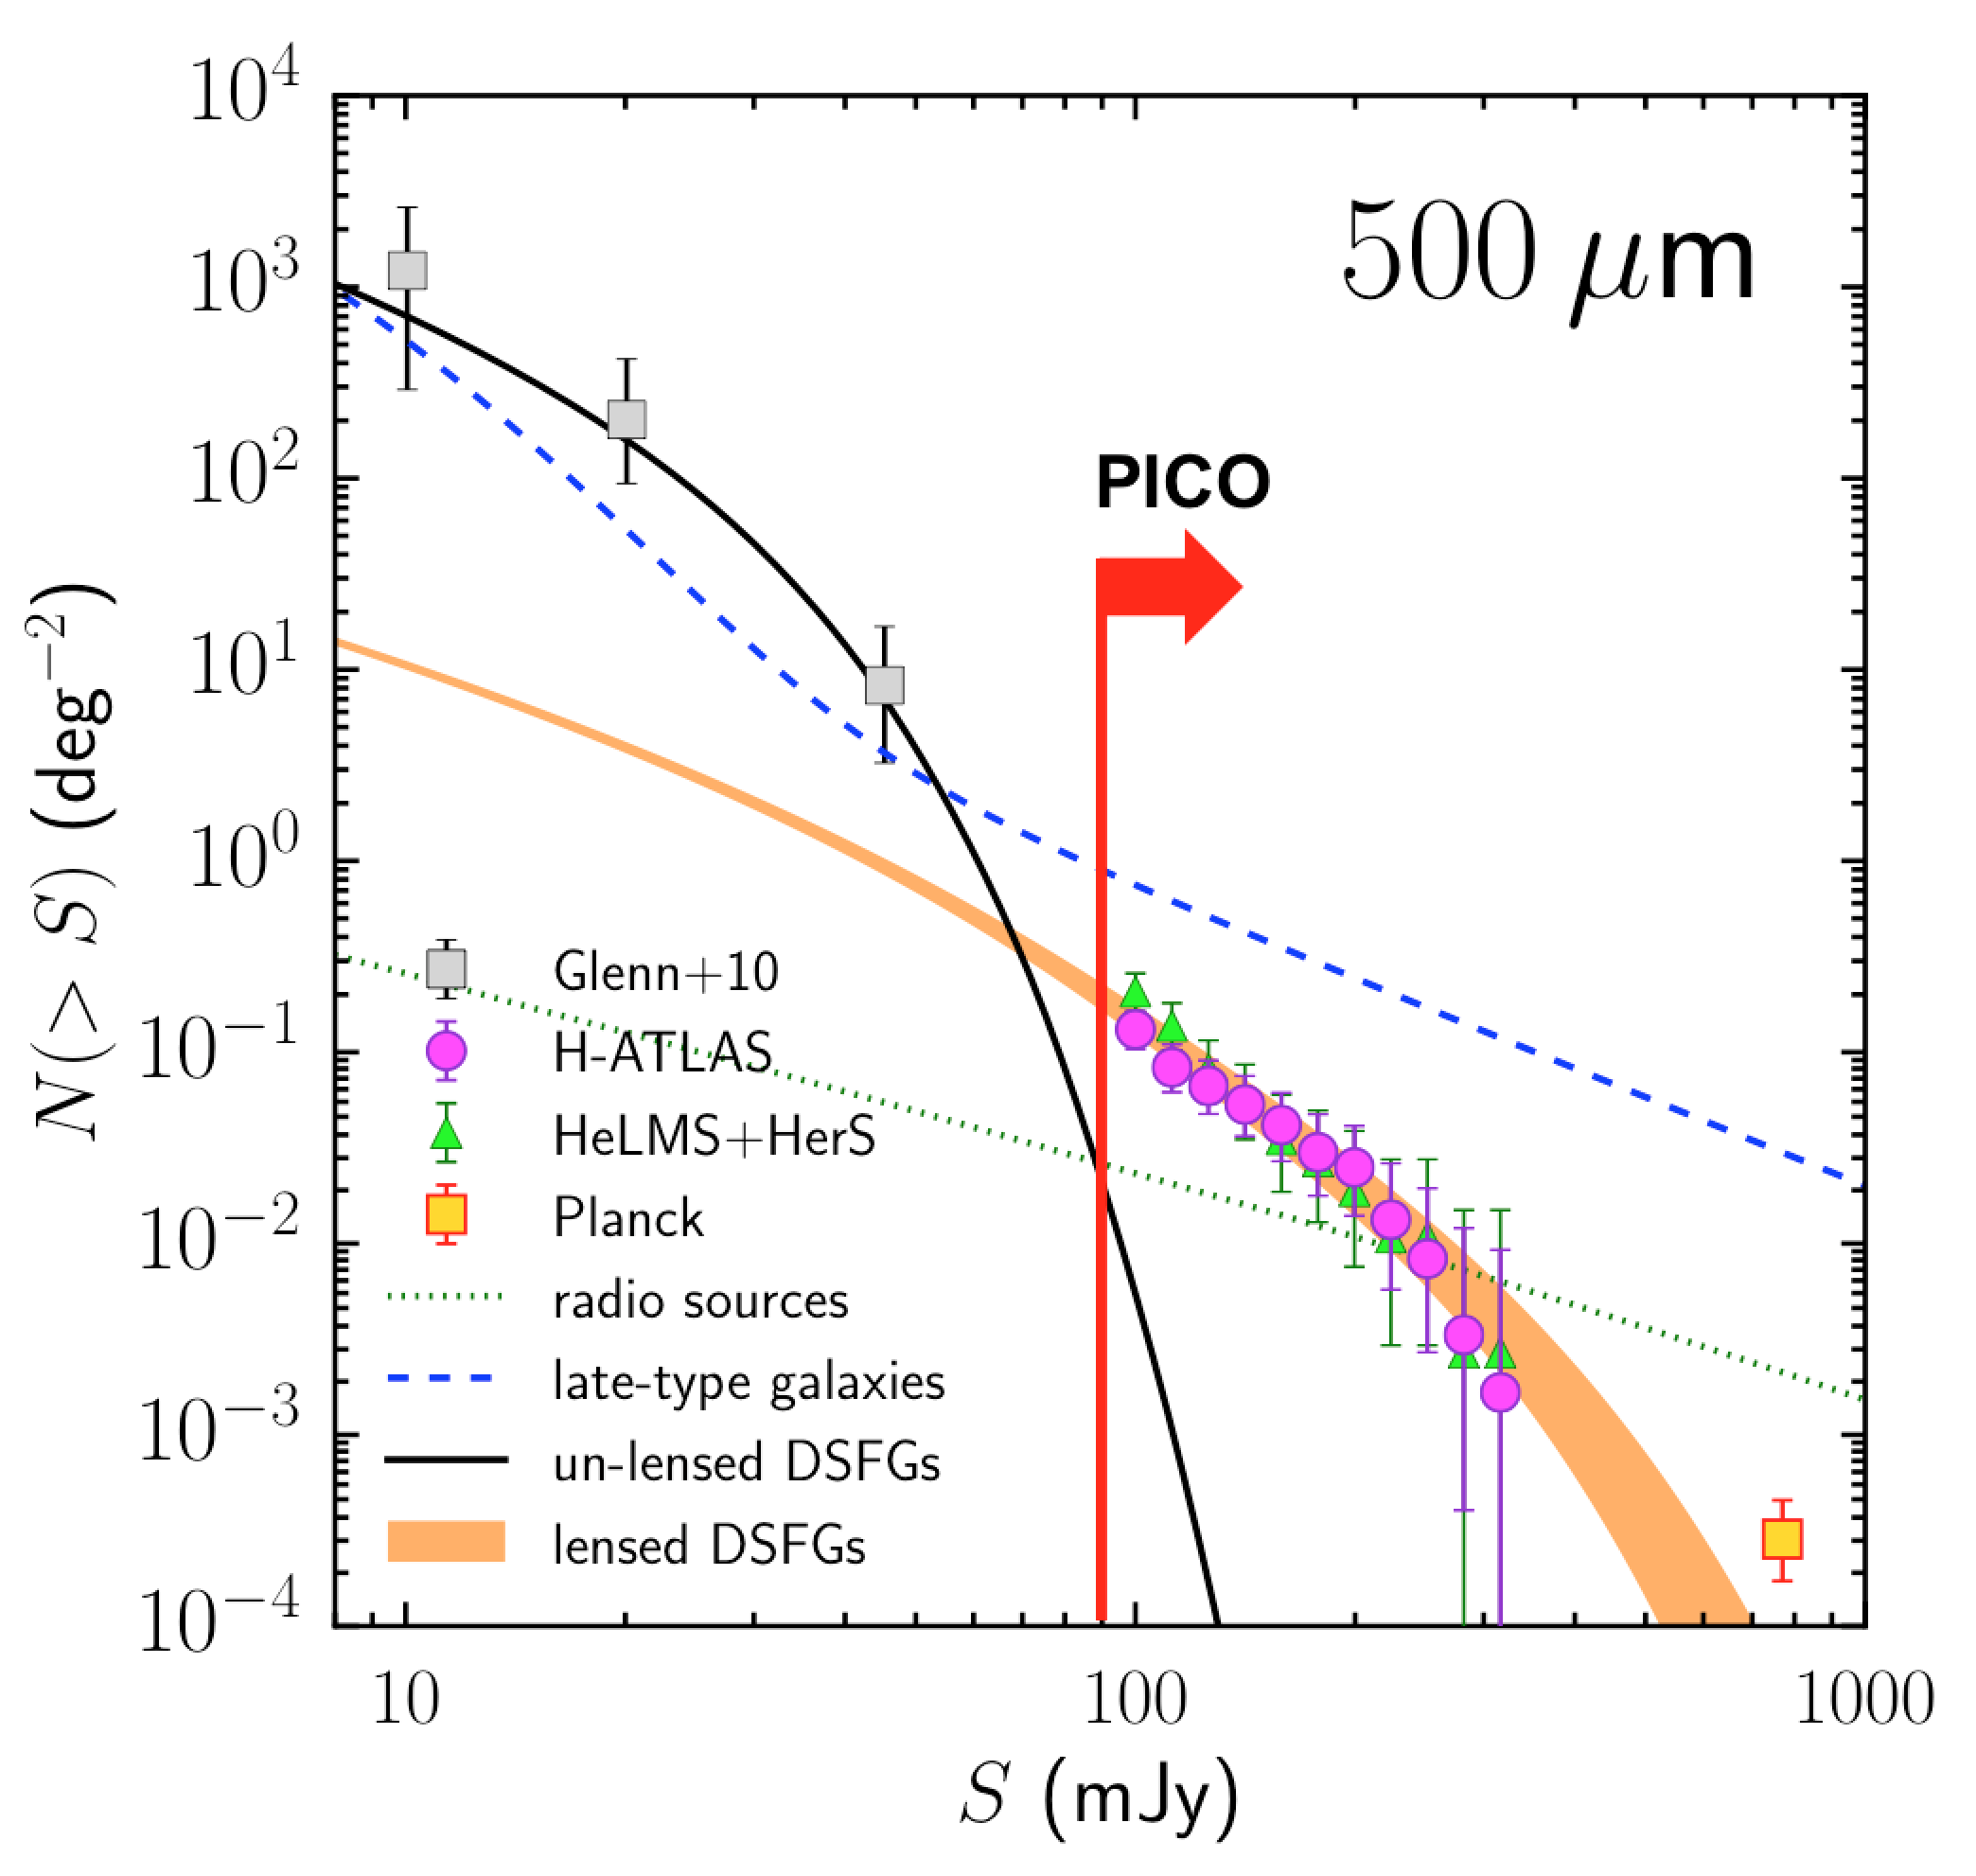
\includegraphics[width=0.48\columnwidth, height=5.5truecm, trim={0 0 0 0cm}, clip]{NgtF_500micron.png}
\caption{\textbf{Left panel.} Examples of SEDs of extragalactic sources detectable by PICO, compared with its point source detection limits (solid black line). The SED of M\,61 has been scaled down by a factor of 10. The 90\% completeness limits of the Second \textit{Planck} Catalogue of Compact Sources (PCCS2; \cite{PCCS2}) are also shown.  \textbf{Right panel.} Integral counts of the various populations of extragalactic sources at $500\,\mu$m as determined by \textit{Herschel} surveys. The vertical red line shows the estimated PICO detection limit.}
\label{fig:SED3}
\end{center}
\end{figure*}

\subsection{Point extragalactic sources in the PICO frequency range}

As illustrated by the left panel of Fig.\,\ref{fig:SED3}, at $\lambda \simgt \hbox{few\, mm}$ the dominant extragalactic population are blazars (flat-spectrum radio quasars, FSRQs, and BL Lacs), typically at $z\simgt 1$; the solid blue line shows an example. At shorter wavelengths dusty galaxies take over. The brightest sources in this spectral range are nearby  star-forming galaxies like M\,61. PICO will also see the brightest high-$z$ sub-mm sources which, due to the ``magnification bias'', are those whose flux density is boosted by strong gravitational lensing.

\textit{Herschel} surveys have shown that, at $500\,\mu$m (600\,GHz), about 20\% of galaxies at the PICO detection limit are strongly lensed (right panel of Fig.\,\ref{fig:SED3}). This is an extraordinary selection efficiency: for   comparison, the fraction of strongly lensed galaxies is of $\sim 10^{-3}$ in all other frequency bands where searches have been carried out. Also, these galaxies have sub-mm colors substantially different from those of the other extragalactic populations and are therefore very easily singled out \cite{Negrello2017lensed}.

PICO will detect several thousands strongly lensed galaxies. Objects like the $z=4$ source HLSJ$091828.6+514223$ (left panel of Fig.\,\ref{fig:SED3}; \cite{Combes2012}) would be detectable by PICO up to extreme redshifts ($z>10$).

The availability of thousands of strongly lensed galaxies opens exciting prospects both on the astrophysical and on the cosmological side (cf., e.g., ref. \cite{Treu2010}). Compared to searches in other wavebands, PICO detections will extend to much higher redshift sources \cite[most optically-selected strongly lensed galaxies are at $z<1$, cf. Fig.\,7 of ref. ][]{Treu2010} and will pick up the rare most extreme amplifications, thanks to its all sky coverage: the magnification factors, $\mu$, of ``\textit{Planck} dusty GEMS'' are estimated to be of up to 50 \cite{Canameras2015}.

Sub-mm lensing allows us to probe the most active star-formation phases, hardly visible in the optical. The gravitational flux boosting is accompanied by a stretching of images. Thus follow-up  with ALMA can achieve an effective resolution of several milli-arcsec, i.e. can measure galactic structures at $z\simeq 3$ down to the astounding level of $\sim 50-60\,$pc, much smaller than the sizes of Galactic giant molecular clouds \cite{Canameras2017ALMA}. This provides unique direct information on the mechanisms driving the star-formation  and on the shapes, sizes and surface brightnesses of star-formation regions.

The detection of several thousands of galaxies at redshifts $\simgt 1$ and up to $z>5$ allows a substantial progress towards a complete census of the dust-enshrouded star-formation history of the universe, i.e. towards tracking the buildup of stellar mass over cosmic time, in particular over epochs of most intense star formation.

The high redshifts of magnified galaxies imply high redshifts of  foreground lenses. Optical follow-up will allow us to investigate the total (visible and dark) mass of the lensing galaxies, their density profiles, dark matter sub-structures in a much higher redshift range than in the case of optical selection \cite{Canameras2017lens}.

Also PICO will explore essentially the entire Hubble volume for the most intense hyperluminous starbursts, testing whether there are physical limits to the star-formation rates of galaxies.

The right panel of Fig.\,\ref{fig:SED3} also shows that PICO will detect tens of thousands star forming galaxies in the nearby universe, reaching a surface density about a factor of two higher than that of the IRAS satellite at its $60\,\mu$m completeness limit \cite{RowanRobinson1991}. The IRAS
wavebands  are relatively insensitive to low temperature dust emission,
a significant and largely unexplored component of many nearby galaxies \cite{Planck2011nearby_gal}. PICO will provide a full characterization of this component, complementing IRAS data to establish well calibrated dust SEDs as a function of galaxy morphology, luminosity, dust and gas mass, etc..


\begin{figure*}
%\vskip-6cm
\begin{center}
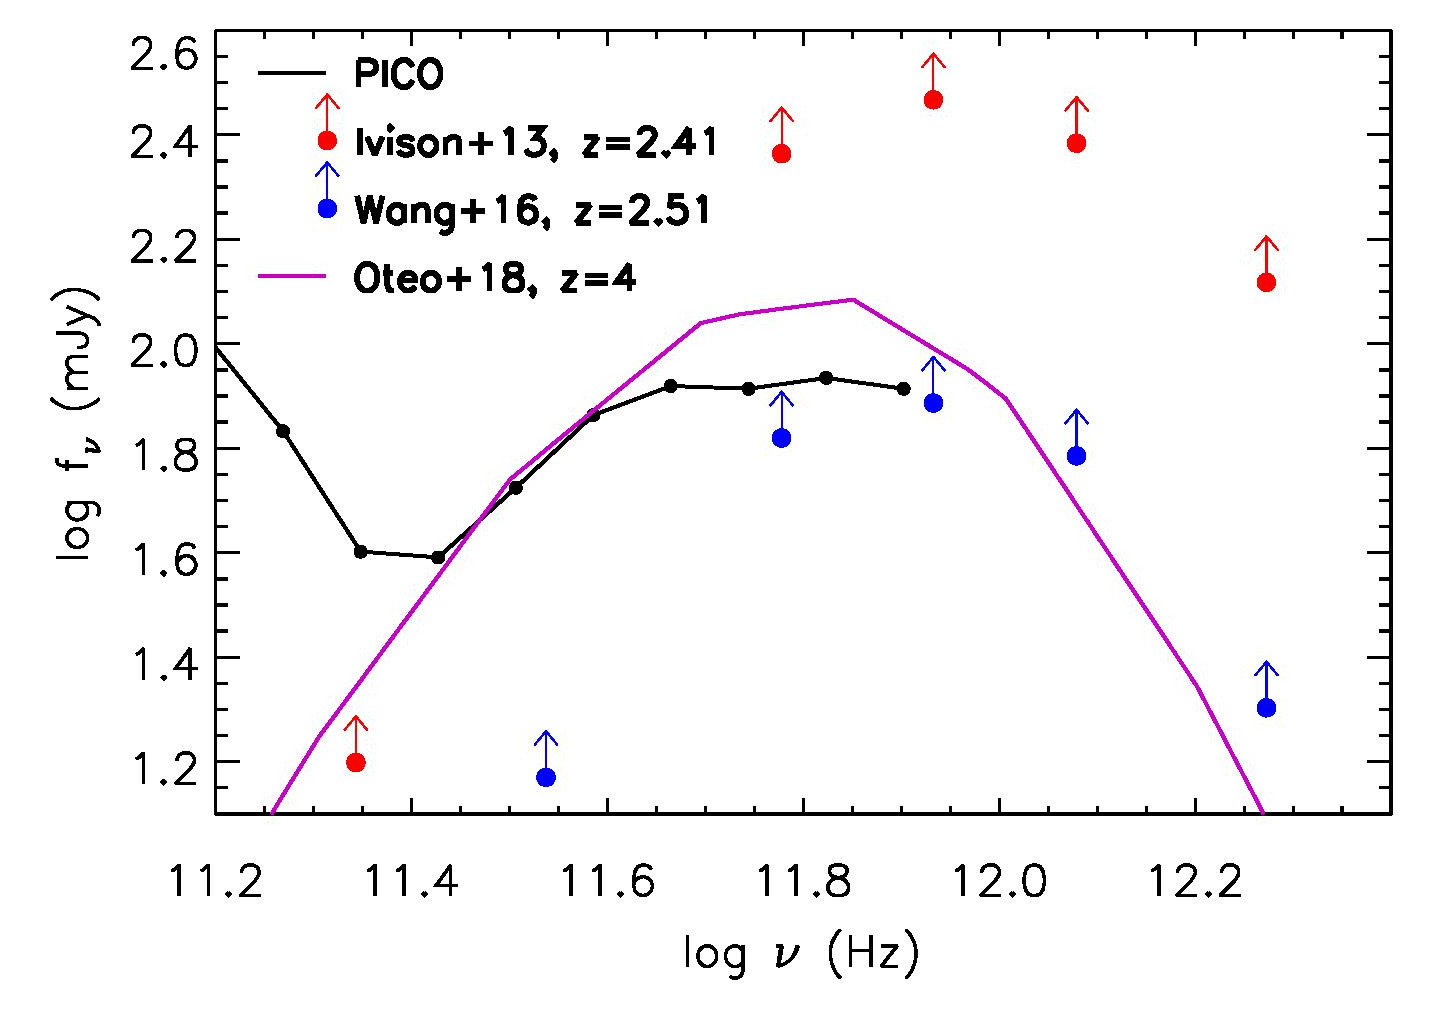
\includegraphics[width=0.32\columnwidth, trim={0 0 0 0cm}, clip]{fig_protocl_PICO}
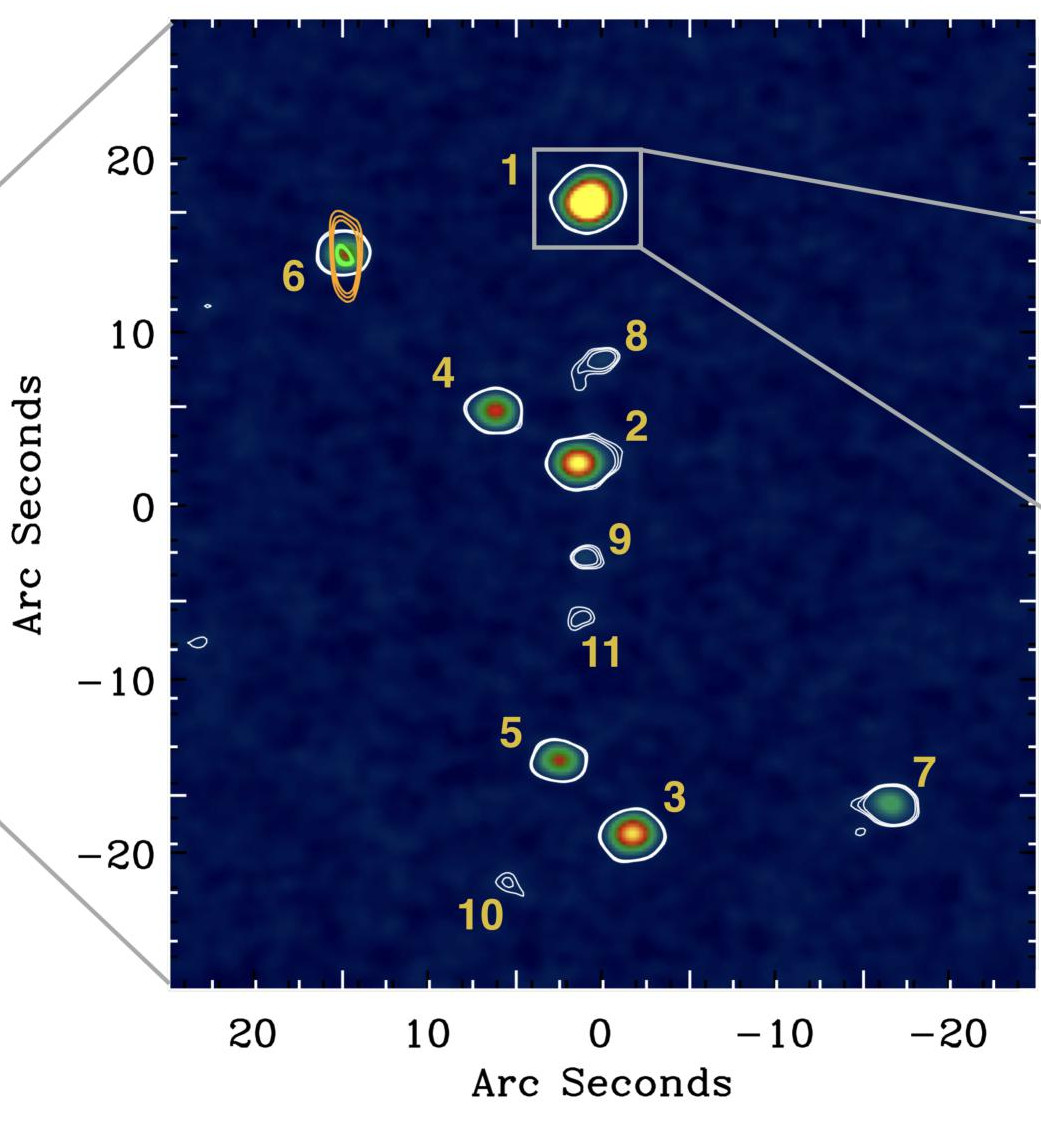
\includegraphics[width=0.32\columnwidth, height=3.7truecm, trim={0 0 0 0.cm}, clip]{Oteo_2018_protocl.jpg}
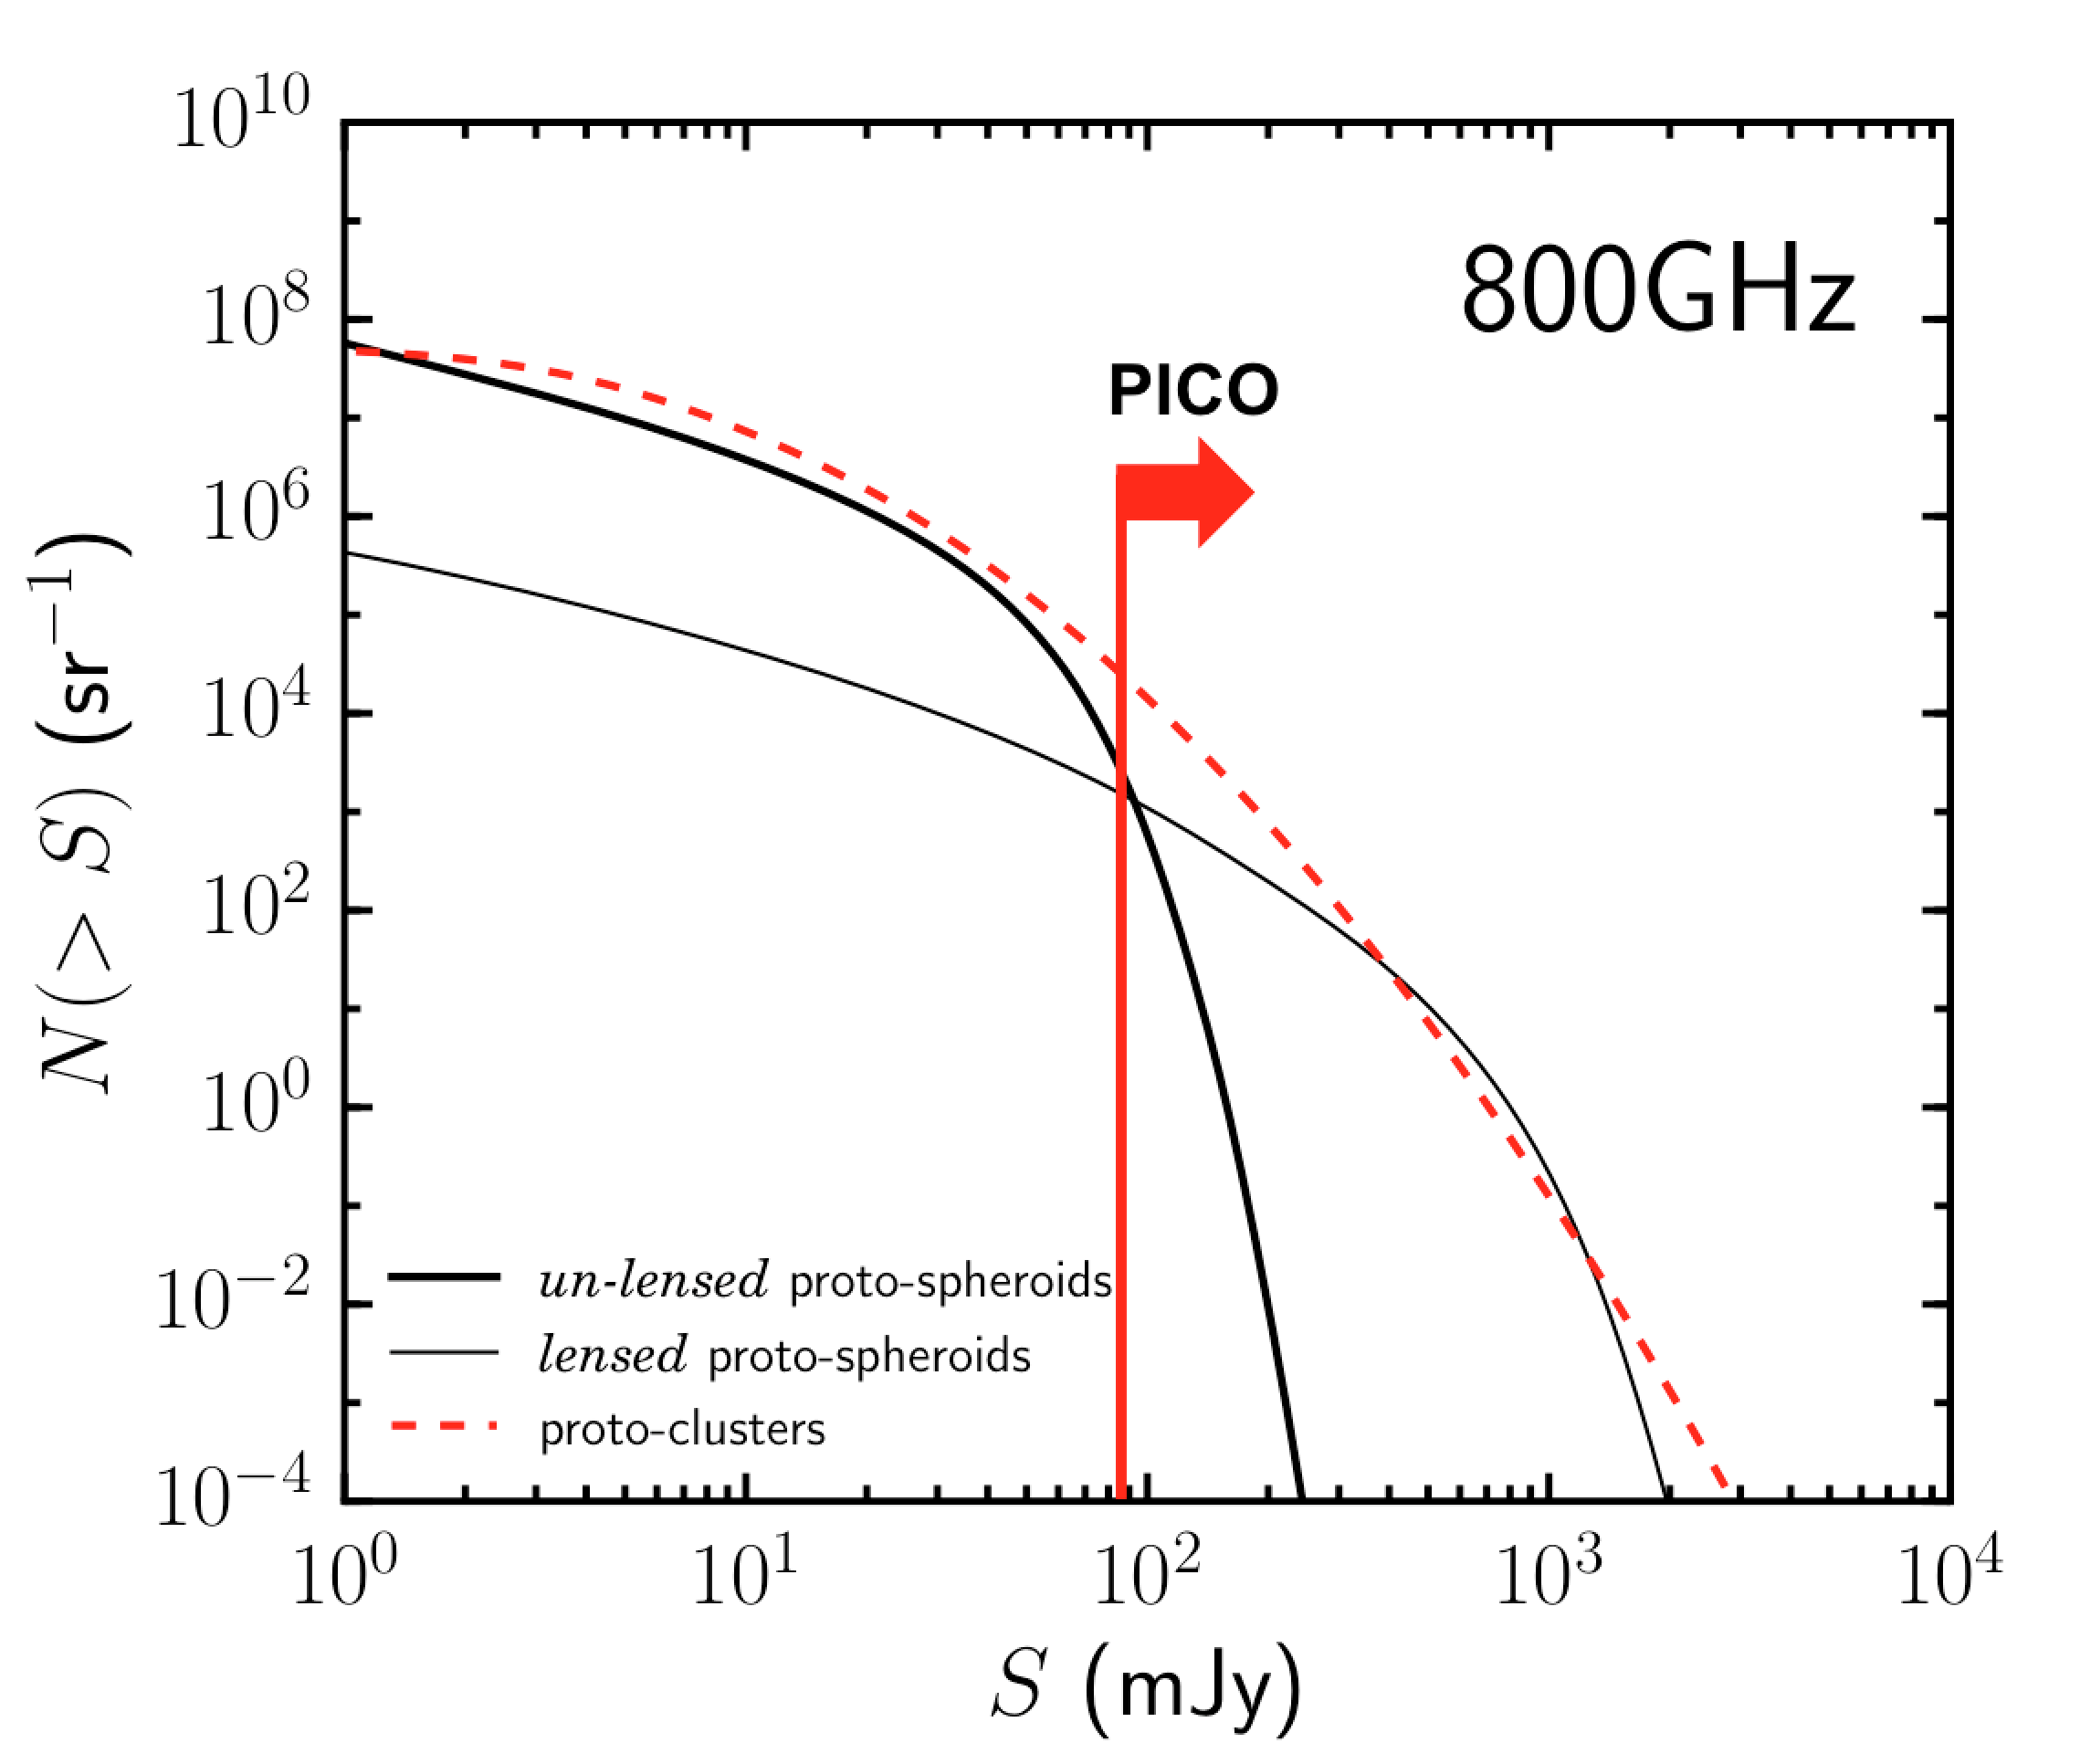
\includegraphics[width=0.32\columnwidth, height=3.7truecm, trim={0 0 0 0.cm}, clip]{NgtFclumps_800GHz.png}
%\includegraphics[width=0.48\columnwidth, trim={0 0 0 0.cm}, clip]{dNdzclumps_600GHz.jpg}
\caption{\textbf{Left panel.} SEDs of the cores of two proto-clusters of starbursting galaxies  discovered by \cite{Ivison2013} at $z=2.41$, by \cite{Wang2016} at $z=2.506$ and by \cite{Oteo2018} at $z=4.0$. The first two SEDs include only the contributions of proto-cluster members within $10''$, i.e. over an angular size below the PICO resolution, corresponding to physical radii $\simeq 80\,$kpc, substantially smaller than the effective proto-cluster sizes. The reported flux densities are therefore lower limits to those that will be measured by PICO. The SED of the $z=4.0$ proto-cluster correspond to a SFR of $6500\,M_\odot\,\hbox{yr}^{-1}$, estimated by \cite{Oteo2018} summing the contributions of galaxies detected by ALMA within a radius of $\simeq 25''$; again this is likely a lower limit to what PICO will measure. The solid black line shows the PICO detection limits. \textbf{Central panel.} ALMA image of the $z=4.0$ proto-cluster discovered by \cite{Oteo2018}, extracted from Fig.~1 of their paper. \textbf{Left panel.} Counts of proto-clusters at 800\,GHz predicted by the  model of ref. \cite{Negrello2017protocl}. The vertical red line corresponds to the PICO detection limit.
%\textbf{Lower right panel.} Predicted redshift distribution of proto-clusters above the PICO detection limit at 800\,GHz.
}
\label{fig:protocluster}
\end{center}
\end{figure*}


\subsection{Early phases of cluster evolution}

PICO will open a new window for the investigation of early phases of cluster evolution, when their member galaxies were actively star forming and before the hot IGM was in place. In this phase traditional approaches to cluster detection (X-ray and SZ surveys, searches for galaxy red sequences) work only for the minority of evolved objects; indeed they have yielded only a handful of confirmed proto-clusters at $z\simgt 1.5$ \cite{Overzier2016}\footnote{More high-$z$ proto-clusters have been found targeting the environment of tracers of very massive halos, such as radio-galaxies, QSOs, sub-mm galaxies. These searches are however obviously biased.}.

SEDs of spectroscopically confirmed sub-mm-bright proto-clusters detectable by PICO are shown in the left panel of Fig.~\ref{fig:protocluster}). \textit{Planck} has demonstrated the power of low-resolution surveys for the study of large-scale structure  \cite{Planck2016high_z} but its resolution was too poor to detect individual proto-clusters \cite{Negrello2017protocl}.
As illustrated by the central panel of Fig.~\ref{fig:protocluster}, the typical sizes of high-$z$ proto-cluster cores are of $\sim 1'$ (cf. also ref. \cite{Alberts2014}), nicely matching the PICO FWHM at the highest frequencies.

CMB Probe will detect many tens of thousands of these objects (right-hand panel of Fig.~\ref{fig:protocluster}) up to $z\simgt 4$ (left panel). This will allow a real breakthrough in the observational validation of the formation history of the most massive dark matter halos, traced by clusters, a crucial test of models for structure formation. Follow-up observations will characterize the properties of member galaxies, probing the galaxy evolution in dense environments and shedding light on the complex physical processes driving it.

\subsection{Radio sources}

PICO will increase by orders of magnitude the number of blazars selected at sub-mm wavelengths and will determine the SEDs of many hundreds of them up to 800\,GHz. The most luminous high-$z$ FSRQs were found to host black holes (BHs) with the largest masses, up to $\sim 4\times 10^{10}\,M_\odot$ (S$5\,0014+813$, at  $z = 3.366$; see ref. \cite{Ghisellini2009}). Such objects have particularly hard mm-wave spectra; thus PICO surveys are well suited to detect them. Objects like S$5\,0014+813$ are detectable by PICO up to $z>5$.

Blazar searches are the most effective way to sample the most massive BHs at high $z$ because of the Doppler boosting of their flux densities. Since the flux boosting occurs for jets closely aligned with the line of sight ($\theta < 1/\Gamma$, $\Gamma \sim 15$ being the bulk Lorentz factor), for each FSRQ there are other $2\Gamma^2$  (i.e. hundreds) sources of similar intrinsic properties but pointing elsewhere.

Very large BH masses at high-$z$ challenge models because it is very hard to grow a seed BH from stellar mass to $> 10^9\,M_\odot$ in the limited age of the universe. It is even more so for jetted quasars because jets are likely associated with rapidly spinning BHs whose radiative efficiency is large so that the mass growth is slow. Yet at least 4 FSRQs has been discovered at $z>5$ (up to $z=5.48$; \cite{Romani2004}). One (SDSS J$013127.34–032100.1$ at $z = 5.18$) has estimated BH mass of $\sim 10^{10}\,M_\odot$ \cite{Ghisellini2015}.

The PICO surveys of the largely unexplored mm/sub-mm spectral region will also offer the possibility to discover new transient sources \cite{Metzger2015} or events, such as blazar outbursts.

%\begin{figure}
%\vskip-3cm
%\includegraphics[width=\columnwidth]{./COrE_pol_detections_both.png}
%\caption{Comparison of the estimated source number counts in polarization for a selection of CORE channels and different source populations: radio sources (solid blue line); and two populations of dusty galaxies (proto-spheroids and late-type, spiral and starburst, galaxies). Proto-spheroids, labelled ``High-z IR'' (solid green line) dominate at faint flux densities while late-types  (LT IR, solid red lines) dominate at the brighter flux densities. The vertical lines show the $4\sigma$ and  $5\sigma$ detection limits obtained from the simulations for the 1-m ({dashed}) and 1.5-m ({solid}) telescope. From \citet{DeZotti2016}.}
%\label{fig:both}
%\end{figure}

\subsection{Source polarization}

PICO will make a giant leap forward in the determination of
polarization properties of both radio sources and of dusty galaxies over a
frequency range where ground based surveys are impractical or impossible.
Thanks to its high sensitivity, it will detect in polarization both populations over a substantial flux density range, determining directly, for the first time, number counts in polarized flux density.

Mm/sub-mm polarimetry of radio sources provides unique information on the magnetic field configuration (geometry and degree of order) in the innermost, unresolved regions of the jets, close to the active nucleus. Polarimetry of dusty galaxies as a function of their inclination is informative on the structure and on the ordering of their large-scale magnetic fields.



\newpage



\bibliography{mybib}

\end{document}

%%%%%%%%%%%%%%%%%%%%%%%%%%%%%%%

